% Standalone bar chart for Section 2: exact enumeration counts across the three domains.
\documentclass[tikz,border=3pt]{standalone}
\usepackage{pgfplots}
\pgfplotsset{compat=1.17}
\definecolor{cState}{HTML}{AABEDA}
\definecolor{cAssert}{HTML}{2E6DA4}
\definecolor{cFeas}{HTML}{4C9A4C}
\begin{document}
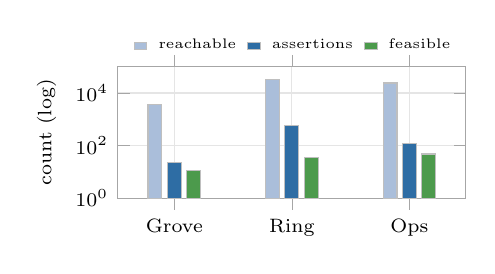
\begin{tikzpicture}
\begin{axis}[
  ybar, bar width=5pt, ymode=log, area legend,
  legend image code/.code={\draw[#1] (0cm,-0.045cm) rectangle (0.16cm,0.045cm);},
  width=6.0cm, height=3.25cm,
  ymin=1, ymax=1e5,
  symbolic x coords={Grove,Ring,Ops}, xtick=data,
  enlarge x limits=0.24,
  ytick={1,100,10000},
  tick label style={font=\scriptsize},
  x tick label style={font=\scriptsize},
  ylabel={count (log)}, ylabel style={font=\scriptsize},
  legend style={font=\tiny, at={(0.02,1.02)}, anchor=south west,
    legend columns=3, draw=none, fill=none, /tikz/column sep=2pt},
  legend cell align=left,
  grid=major, major grid style={black!10},
  axis line style={black!35},
  tick style={black!35},
]
\addplot[fill=cState, draw=black!25] coordinates
  {(Grove,3631) (Ring,32928) (Ops,23978)};
\addlegendentry{reachable}
\addplot[fill=cAssert, draw=black!25] coordinates
  {(Grove,22) (Ring,576) (Ops,120)};
\addlegendentry{assertions}
\addplot[fill=cFeas, draw=black!25] coordinates
  {(Grove,11) (Ring,36) (Ops,48)};
\addlegendentry{feasible}
\end{axis}
\end{tikzpicture}
\end{document}
